\section{Method}

% We introduce Light LLM-Guider, a lightweight knowledge distillation method that treats LLM as a black-box and transfer its superior semantic alignment ability to reranker models and hence the performance of the retriever model within retrieval-augmented generation framework.

% 0112 delete
% Previous work in information retrieval often uses a ranker model to refine the order of information retrieved by the retriever model, aiming to improve the accuracy of the top results.
% In this work, we utilize the ranker model differently, using it as an intermediary for knowledge distillation from LLMs to the retriever model, as letting LLMs perform relevance-based ranking tasks for ranker training is simpler and more robust than having them directly generate a relevance likelihood for retriever training.

% we adapt this two-stage workflow, using a ranker model as an intermediary for knowledge distillation from LLMs to the retriever model instead of as a way to enhance the results' accuracy.
% As discussed in the previous sections, letting LLMs perform relevance-based ranking tasks is simpler and more robust than having them predict or directly generate a quantified likelihood of information relevance.

Our two-stage distillation scheme uses a ranker model and a retriever model as the student models and a LLM as the teacher model.
As shown in Figure \ref{fig:02}, we initially employ an off-the-shelf retriever to select a subset of documents $D_n$ from a large corpus $D$ based on their relevance to a query $Q$.
The LLM then re-ranks these documents, creating a ranking order $\pi$, which is used to train the ranker model in the distillation \textit{Stage 1}.
In \textit{Stage 2}, this ranker enhances the original retriever by minimizing the KL-divergence between their similarity likelihood.
% The following sections introduce our proposed framework in details, and is organized as follows.
In detail, Section \ref{sec:3-1} provides the formal definitions of the related tasks. 
In Section \ref{sec:3-2} and Section \ref{sec:3-3}, we show how knowledge is directly transferred from LLMs to a ranker model and then further conveyed to a retriever model, respectively.


\subsection{Problem Formulation}
\label{sec:3-1}
Given a question $Q$, the goal of a retriever model is to find a subset of the most relevant documents $D_n=\{n_1, n_2, ..., n_k\} \subseteq D$ from a large knowledge corpus $D=\{d_1, d_2, ..., d_m\}$, where each $d_i, n_i$ represents a unique document.
In the retrieval-augmented generation (RAG) framework, this subset $D_n$ is combined with the question $Q$ to form the reader's prompt input and then generates the corresponding answer $A$.

For the re-ranking task in our distillation framework, the teacher ranker model (i.e., LLMs) is tasked with reordering the documents $D_n$ according to their relevance to the question $Q$.
The re-ranking order can be represented as $\pi: T_{sim}(n_i, Q)>T_{sim}(n_k, Q) > ... > T_{sim}(n_j, Q)$, indicating the descending order of relevance from the documents $n_i, n_j, ..., n_k$ in the subset $D_n$.
This order information $\pi$ is first transferred to the ranker model, which serves as an intermediary between the LLM and the retriever model.
Subsequently, the ranker model conveys this knowledge to the retriever, thereby enhancing its performance.
% and serve as an intermediary to transfer the knowledge from LLMs to the retriever model finally.

\begin{figure*}
    \centering
    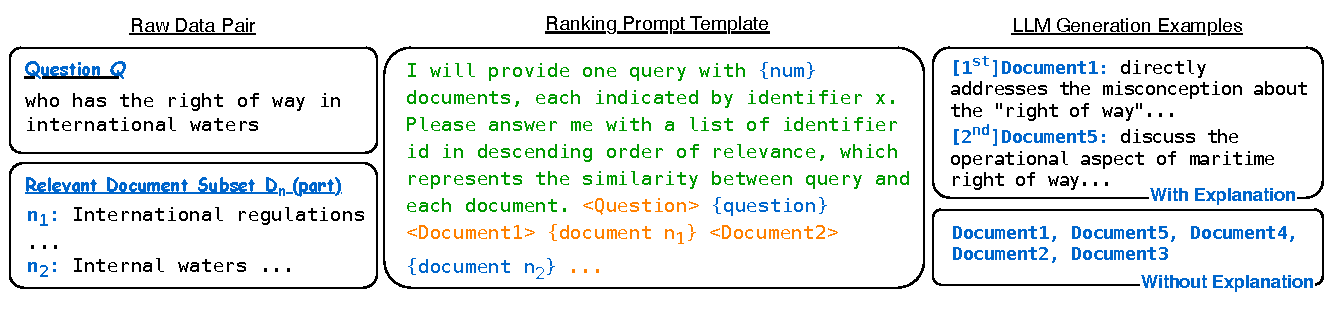
\includegraphics[width=1.0\textwidth]{latex/pic/fig3.pdf}
    \caption{An example of our LLM teacher model's re-ranking process.}
    \label{fig:03}
    % \vspace{-3mm}
\end{figure*}

\subsection{Stage 1: Distillation from LLMs to Ranker} 
\label{sec:3-2}
% \textbf{Ranking Data Initialization} 
The initial step of our knowledge distillation workflow is data initialization, where we find the relevant document subsets $D_n$ from corpus $D$ for each specified question $Q$. 
These subsets then serve as the input for the \textit{Stage 1} training.
In practice, we employ a widely-used information retrieval model, Contriever \cite{izacard2022unsupervised}, as the retriever model for data initialization. \\
% Additionally, we initialize both the ranker and retriever models within our distillation framework using off-the-shelf Contriever model checkpoints.\\
\textbf{Re-ranking by LLMs.} 
In this stage, we utilize LLM's guaranteed zero-shot ranking capabilities to generate high-quality re-ranking orders for each subset $D_n$ based on the relevance to the corresponding question $Q$.
We use a list-wise ranking prompt, which is adapted from the RankGPT \cite{sun2023chatgpt}, as our input ranking prompt.
Figure \ref{fig:03} illustrates a LLM re-ranking process, where the LLM generates a re-ranking order $\pi_{D_n}: T_{sim}(n_1, Q)>T_{sim}(n_5, Q) >T_{sim}(n_4, Q) > T_{sim}(n_3, Q) > T_{sim}(n_2, Q)$. 
% We found that the LLM's excellent semantic alignment capabilities effectively pushed documents containing the corresponding answers to higher positions in the generated responses, as shown in Table 2 (where the numbers represent the average ranking position of documents containing the answers). 
Following this, we use these re-ranking orders to transfer LLM's knowledge into a smaller but more efficient ranker model.
 \\
\textbf{Ranker Distillation Training}
We initialize our ranker model by using the dual-encoder structure \textit{Contriever} checkpoint.
% To extract the ranker model's representation of the similarity between each document $n_i \subset D_n$
For each question $Q$ and its retrieved document $n_i \subseteq D_n$, we represent the question and document using the average value from the last hidden layer of the ranker model, denoted as $\hat{Q}$ and $\hat{n}_i$, respectively.
For each training data instance, once we have the representative embeddings $\hat{Q}$ and $\hat{n}_i$, we proceed to calculate the similarity likelihood $P_{RANK}$ over $D_n$, which can be defined as:
\begin{equation}
    P_{RANK}(n_i|Q) = \frac{exp(s(\hat{n}_i, \hat{Q})/\theta)}{\sum_{k=1}^Kexp(s(\hat{n}_k, \hat{Q})/\theta)}
\end{equation}
where $s$ denotes the dot-product between the ranker's representation vectors of the question and each retrieved document, and $\theta$ is the temperature hyper-parameter.
% \textbf{Ranker Training Objective} 

After obtaining the ranker model's similarity likelihood $P_{RANK}(n_i|Q)$ over its relevant document subset $D_n$, and the LLM-generated re-ranking order $\pi_{D_n}$, we use ListMLE \cite{xia2008listwise}, a list-wise loss function for distillation training from LLMs to the ranker model.
ListMLE considers the similarity likelihood $P_{RANK}(D_n)$ as the predicted list and $\pi_{D_n}$ as the ground truth, aiming to minimize the following loss function:
% where oi is the quality order of the i-th sentence measured by M . N1 is the number of sentences.
% \begin{equation}
%     L(f(x), y) = -log(P({\pi_{f(x)}}|y))
% \end{equation}
\begin{equation}
    \begin{aligned}
    L(P_{RANK}, \pi) 
    &= -log P(\pi_{P_{RANK}}|\pi) \\
    &= -log \prod _{j=1}^k \frac{exp(P_{RANK}(n_i))}{\sum_{m=j}^kexp(P_{RANK}(n_m))}
    \end{aligned}
\end{equation}
where $\pi_{P_{RANK}}$ represents the permutation of documents ordered by the ground truth ranking $\pi$. 
The loss function calculates an exponential probability distribution over all elements of $P(\pi_{P_{RANK}}|\pi)$, expressing the loss as the negative log-likelihood of the ground truth order $\pi$.
% and calculates the cumulative product across the sequence as defined by $\pi_{p_{RANK}}$.
% and $P({\pi_{f(x)}}|y)$ is the Plackett-Luce probability of a permutation $\pi_{f(x)}$ conditioned on scores $y$.
% Here we apply the exponential function to $P({\pi_{f(x)}}|y)$, which is:
% \begin{equation}
%     P({\pi_{f(x)}}|y) = \prod _{j=1}^n \frac{e^{f(x_i)}}{\sum_{k=j}^ne^{f(x_k)}}
% \end{equation}
% whose cumulative multiplication follows the permutation order $\pi$.
\subsection{Stage 2: Distillation from Ranker to Retriever}
\label{sec:3-3}
% After completing Stage 1 of our proposed framework, we obtain a well-trained ranker model. 
In \textit{Stage 2}, this well-train ranker model is used to enhance the retriever model's performance by transferring knowledge from LLMs.\\
% \textbf{Compute Retriever Similarity Likelihood.} 
We initialize our retriever model using a dual-encoder Contriever checkpoint, similar to the ranker.
For each question and its retrieved document, we also compute their representations $\widetilde{Q}$ and $\widetilde{n}_i$ by calculating the average value from the retriever model's last hidden layer and the similarity distribution $P_{RETR}$ of the retriever model over $D_n$ is defined as:
\begin{equation}
    P_{RETR}(n_i|Q) = \frac{exp(s(\widetilde{n}_i, \widetilde{Q})/\theta)}{\sum_{k=1}^Kexp(s(\widetilde{n}_k, \widetilde{Q})/\theta)}
\end{equation}
where $s$ represents the dot-product between the retriever's representation vectors of the question and each retrieved document, and $\theta$ is the temperature hyper-parameter.

% \textbf{Retriever Training Objective} 
We then leverage the similarity likelihood $P_{RANK}$ from the previously trained ranker model to enhance the retriever model's performance under an unsupervised learning process by minimizing the KL-divergence between $P_{RANK}$ and $P_{RETR}$:
\begin{equation}
    D_{KL}(P_{RANK}||P_{RETR})
\end{equation}

This process ensures the retriever model aligns more closely with the text similarity knowledge from the LLMs.
Through this two-stage distillation scheme, we enhance the retrieval accuracy and effectiveness of the retriever model, which can be further applied to the RAG framework to improve its performance on knowledge-intensive NLP tasks.